\documentclass{article}

\usepackage{graphicx}
\usepackage{tikz}
\usepackage{tikzsymbols}
\usetikzlibrary{calc,patterns,shapes.geometric}
\pagestyle{empty}
\usepackage[margin=0pt]{geometry}
\geometry{papersize={14in,12in}}

\def\centerarc[#1](#2)(#3:#4:#5){\draw[#1] ($(#2)+({#5*cos(#3)},{#5*sin(#3)})$) arc (#3:#4:#5);}

\begin{document}
	\begin{figure}
		\centering
		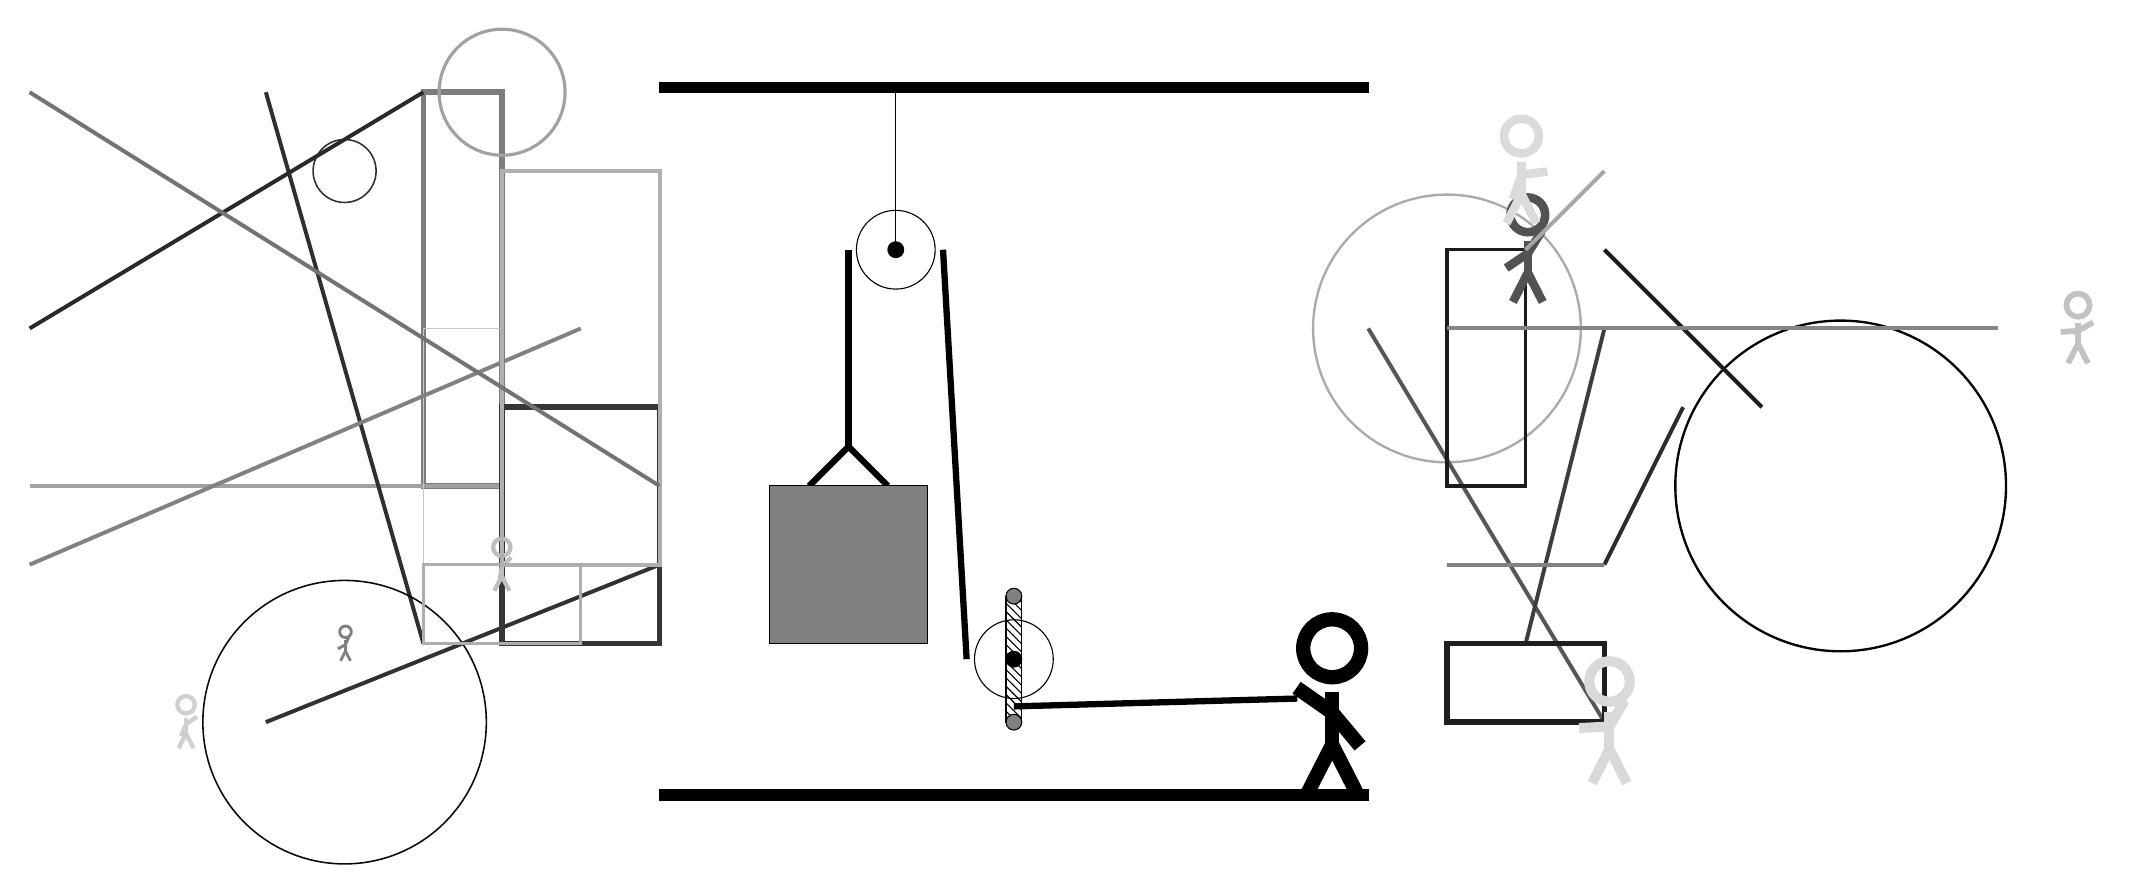
\begin{tikzpicture}
			%%%%% START %%%%%
			
			\draw[fill=black] (-2, 9) rectangle (7, 9.125);
			
			\draw (1, 7) circle (0.5);
			\draw[fill=black] (1, 7) circle (0.1);
			\draw (1, 9) -- (1, 7);
			
			\draw[line width=0.3mm, color=black!79] (-4, 5) rectangle (-4, 5);
			
			\draw [line width=0.3mm, color=black!33](8, 6) circle (1.7);
			\draw[line width=0.5mm, color=black!66](7, 6) -- (10, 1);
			\draw[line width=0.7mm, color=black!51] (-4, 4) rectangle (-5, 9);
			\draw[line width=0.5mm, color=black!76](10, 6) -- (9, 2);
			
			\draw[line width=0.7mm, color=black!88] (8, 2) rectangle (10, 1);
			\draw[line width=0.5mm, color=black!37](-4, 4) -- (-10, 4);
			
			\draw[line width=0.2mm, color=black!22] (-4, 3) rectangle (-5, 6);
			\draw [line width=0.2mm, color=black!81](-6, 8) circle (0.4);
			\draw[line width=0.5mm, color=black!81](-5, 2) -- (-7, 9);
			\draw[line width=0.4mm, color=black!89] (9, 4) rectangle (8, 7);
			
			\draw[line width=0.5mm, color=black!84](-5, 9) -- (-10, 6);
			\node[line width=0.5mm, color=black!15] at (10, 1) {\Strichmaxerl[7][3][60]};
			\node[line width=0.7mm, color=black!68] at (9, 7) {\Strichmaxerl[6][34][58]};
			\draw[line width=0.5mm, color=black!81](-2, 3) -- (-7, 1);
			\draw [line width=0.3mm, color=black!98](13, 4) circle (2.1);
			\draw[line width=0.5mm, color=black!89](10, 7) -- (12, 5);
			
			\draw [line width=0.4mm, color=black!37](-4, 9) circle (0.8);
			\draw[line width=0.5mm, color=black!83](11, 5) -- (10, 3);
			
			\draw[line width=0.5mm, color=black!49](-3, 6) -- (-10, 3);
			\draw [line width=0.2mm, color=black!96](-6, 1) circle (1.8);
			
			\draw[line width=0.7mm, color=black!79] (-2, 2) rectangle (-4, 5);
			\draw[line width=0.5mm, color=black!49] (8, 3) rectangle (10, 3);
			\node[line width=0.2mm, color=black!25] at (-4, 3) {\Strichmaxerl[3][81][45]};
			\draw[line width=0.5mm, color=black!31] (-4, 8) rectangle (-2, 3);
			
			\node[line width=0.6mm, color=black!24] at (16, 6) {\Strichmaxerl[4][3][30]};
			
			\node[line width=0.5mm, color=black!19] at (-8, 1) {\Strichmaxerl[3][67][34]};
			\node[line width=0.4mm, color=black!50] at (-6, 2) {\Strichmaxerl[2][29][67]};
			\draw[line width=0.5mm, color=black!35](9, 7) -- (10, 8);
			
			\node[line width=0.7mm, color=black!14] at (9, 8) {\Strichmaxerl[6][71][7]};
			\draw[line width=0.5mm, color=black!55](-2, 4) -- (-10, 9);
			\draw[line width=0.5mm, color=black!48](8, 6) -- (15, 6);
			\draw[line width=0.4mm, color=black!32] (-3, 2) rectangle (-5, 3);
			
			
			\draw[fill=white](2.5, 1.8) circle (0.5);
			\draw[fill=black] (2.5, 1.8) circle (0.1);
			\draw[pattern=north west lines, pattern color=black] (2.4, 2.6) rectangle (2.6, 1.0);
			\draw[fill=black!50] (2.5, 2.6) circle (0.1);
			\draw[fill=black!50] (2.5, 1.0) circle (0.1);
			
			\draw[line width=0.8mm] (-0.1, 4.0) -- (0.4, 4.5) -- (0.9, 4.0);
			\draw[fill=black!50] (-0.6, 4.0) rectangle (1.4, 2.0);
			
			\draw[line width=0.8mm] (0.4, 7) -- (0.4, 4.5);
			\centerarc[line width=0.8mm](1, 7)(0:180:0.6);
			\draw[line width=0.8mm](1.6, 7) -- (1.9, 1.8);
			\centerarc[line width=0.8mm](2.5, 1.8)(180:270:0.6);
			\draw[line width=0.8mm](2.5, 1.2) -- (6.1, 1.3);
			
			\node at (6.5, 1.2) {\Strichmaxerl[10][-35][-50]};
			
			\draw[fill=black] (-2, 0) rectangle (7, 0.15);
			
			%%%%% END %%%%%
		\end{tikzpicture}
	\end{figure}	
\end{document}